\documentclass{article}
\usepackage[utf8]{inputenc}
\usepackage{geometry}
\geometry{
	a4paper,
	total={170mm,257mm},
	left=20mm,
	top=20mm,
}
\usepackage{graphicx}
\usepackage{titling}
\usepackage{booktabs} % Per linee più belle nelle tabelle
\usepackage{caption}  % Per personalizzare le didascalie
\usepackage{circuitikz}

\title{PRIMA ESPERIENZA DI LABORATORIO.
}
\author{Sebastian Fia, Federico Caposano}
\date{21/10/24}

\usepackage{fancyhdr}
\fancypagestyle{plain}{%  the preset of fancyhdr 
	\fancyhf{} % clear all header and footer fields
	\fancyfoot[L]{\thedate}
	\fancyhead[R]{\theauthor}
}
\makeatletter
\def\@maketitle{%
	\newpage
	\null
	\vskip 1em%
	\begin{center}%
		\let \footnote \thanks
		{\LARGE \@title \par}%
		\vskip 1em%
		%{\large \@date}%
	\end{center}%
	\par
	\vskip 1em}
\makeatother

\usepackage{lipsum}  
\usepackage{cmbright}


\begin{document}
	
	\maketitle   %defined above%
	
	\section{Strumentazione} \label{sec:Strumentazione}
	 	\begin{itemize} 
	 		\item Breadboard
	 		\item Alimentatore da banco (alimentatore duale flottante max/min: +/-30V, 2A; alimentatore singolo flottante max: + 8V, 5A)
	 		\item Multimetro DMM (sensibilità corrente: 200 $\mu$A - 10 A; sensibilità tensione: 200 mV - 1000 V)
	 	
	 	\end{itemize}
	
	\section{Misure di tensione} \label{sec:Tensione}
	\section{Misure di Corrente} \label{sec:Corrente}
	
	
	
	\section{Legge di Ohm} \label{sec:Ohm}
		\subsection{Dati sperimentali}
			\paragraph{}
				Utilizzando il multimetro$^{\ref{sec:Strumentazione}}$ si sono misurate le intensità di corrente (I) al variare arbitrario del voltaggio (V), con una resistenza equivalente di $500\Omega$ ottenuta mettendo in parallelo 2 resistori da $R=1k\Omega$.
				\begin{center}
					\begin{equation}\label{eq:Resistenza}
						R_{eq} = \frac{R^2}{2R}  = \frac{R}{2} = 500\Omega
					\end{equation}
				\end{center}
				
				\begin{center}
					\begin{circuitikz}
						\tikzstyle{every node}=[font=\normalsize]
						
						% Generatore di voltaggio
						\draw (2,10) to[battery, l={\normalsize $V_s$}] (2,7.75);
						
						% Linee orizzontali
						\draw (2,10) to[short] (5.25,10);
						\draw (3.5,7.75) to[short] (5.25,7.75);
						
						% Resistenze
						\draw (5.25,10) to[R, l={\normalsize R}] (5.25,7.75);
						\draw (3.5,10) to[R, l={\normalsize R}] (3.5,7.75);
						
						% Metrica
						\draw (2,7.75) to[rmeter, t=A] (3.5,7.75);
						
						% Nodini
						\node at (3.5,7.75) [circ] {};
						\node at (3.5,10) [circ] {};
					\end{circuitikz}
				\end{center}
				
				
				
				\begin{table}[h]
					\centering
					\captionsetup{skip=10pt} % Imposta lo spazio tra la tabella e la caption
					\caption{MISURE DI LABORATORIO}
					\label{tab:misure_sperimentali}
					\begin{tabular}{c|c}
						V (Volt) & I (mA) \\ \hline
						1 & 1.948  \\ \hline
						2 & 3.998  \\ \hline
						3 & 5.846  \\ \hline
						4 & 7.796  \\ \hline
						5 & 9.747  \\ \hline
						6 & 11.699 \\ \hline
						7 & 13.956 \\ \hline
						8 & 15.955
					\end{tabular}
				\end{table}
		
		
		\subsection{Relazione fra V ed I}
			La legge che mette in relazione la corrente che fluisce in un resistore e la caduta di potenziale che quest' ultimo causa è la \textbf{Legge di Ohm}.
			\begin{equation}
				V = RI
			\end{equation}
			In particolare:
				\begin{equation}
					\frac{V}{I} = R\label{eq:Legge di Ohm}
				\end{equation}
			Dunque fra V ed I c'è una relazione \textbf{lineare}. In cui \textbf{R} è una costante che dipende dalle proprietà fisiche del resistore.
		
		
		\subsection{Stima del valore di R}
		Ipotizzando di non conoscere a priori la $R_{eq}$, dai dati sperimentali e dalla legge di Ohm$^{\ref{eq:Legge di Ohm}}$, si cerca una relazione fra V ed I, del tipo $V/I$.
		
		
			\begin{table}[h]
				\centering
				\captionsetup{skip=10pt} % Imposta lo spazio tra la tabella e la caption
				\caption{CALCOLO R MISURATA}
				\label{tab:calcolo_resistenze}
				\begin{tabular}{r|r|r}
					V (Volt) & I (mA) & $R_i$ ($\Omega$) \\ \hline
					1        & 1.948  & 513.35          \\ \hline
					2        & 3.998  & 500.25          \\ \hline
					3        & 5.846  & 513.17          \\ \hline
					4        & 7.796  & 513.08          \\ \hline
					5        & 9.747  & 512.97          \\ \hline
					6        & 11.699 & 512.86          \\ \hline
					7        & 13.956 & 501.58          \\ \hline
					8        & 15.955 & 501.41         
				\end{tabular}
			\end{table}
		
		Per stimare il valore misurato di R utilizziamo un tool di \textbf{fitting curve} (Vernier Studio), utilizzando un metodo di regressione lineare per calcolare i parametri $b$ e $m$ della retta che meglio approssima la relazione $V/I$.
		
		\begin{figure}[h]
			\centering
			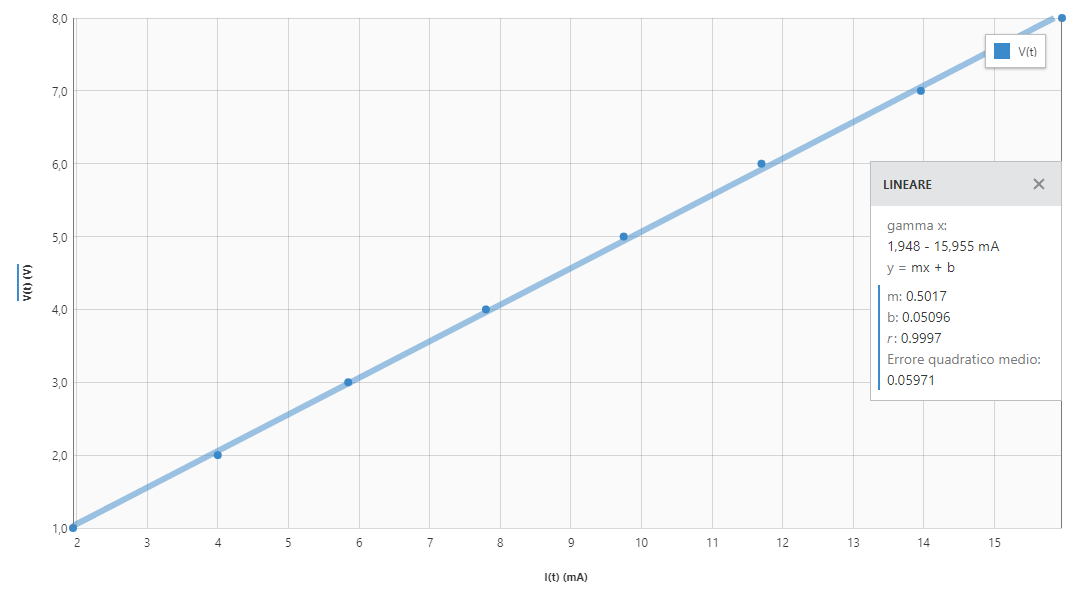
\includegraphics[width=0.75\textwidth]{Graficodiohm.png} % Sostituisci con il nome del tuo file
			\caption{Fitting lineare}
			\label{fig:Grafico}
		\end{figure}
		
		\begin{equation}
			\textbf{Best Fit} \quad\quad\quad\quad	y = 50.9 + 501.7x
		\end{equation}
		
		Il parametro $m$ corrisponde alla misura della resistenza $R_{eq}$, effettivamente la misura coincide con il reale valore della $R_{eq}$.
		
		\begin{equation}
			R_{eq} = 500\Omega \simeq 501.7 = R_{mis}
		\end{equation}
	
	
\end{document}